\documentclass{beamer}

\usepackage{moy-slides}
\usepackage{tikz}
\usepackage{comment}
\usepackage{listings}

\title[Path-focusing]{Static Analysis by Abstract Interpretation, \\ Path Focusing}

%\subtitle{} % (optional)

\author[Julien Henry]{Julien Henry}
% - Use the \inst{?} command only if the authors have different
%   affiliation.

\institute[Verimag]{Grenoble INP Ensimag \\~\\ Tutors: \\ David Monniaux, Matthieu
Moy}

\tikzstyle{arrow}=[->,line width=.05cm,draw=red!90!blue!60!black]

\usetikzlibrary{snakes,arrows,shapes,backgrounds,shadows,automata,patterns}
\usepgflibrary{snakes}

\tikzstyle{state}=[circle,fill=black!25,minimum size=13pt,inner sep=0pt]
\tikzstyle{transition}=[rectangle,thick,draw=black!75,
  			  fill=black!20,minimum size=4mm]
\tikzstyle{transition2}=[rectangle,thick,draw=blue!75,
  			  fill=blue,minimum size=4mm,blue]
\tikzstyle{PRstate}=[circle,fill=red!65,minimum size=13pt,inner sep=0pt]
\tikzstyle{polyhedra}=[blue!25,opacity=0.5,pattern=north west lines,pattern
color=blue]
\tikzstyle{line}=[black,thick]

\date{June 24$^{th}$ 2011}

\newcommand{\backupbegin}{
   \newcounter{framenumbervorappendix}
   \setcounter{framenumbervorappendix}{\value{framenumber}}
}
\newcommand{\backupend}{
   \addtocounter{framenumbervorappendix}{-\value{framenumber}}
   \addtocounter{framenumber}{\value{framenumbervorappendix}} 
}

\lstnewenvironment{C}
{\lstset{language=C,
		basicstyle=\ttfamily,
		commentstyle=\color{moka}\textit,
		keywordstyle=\color{minuit},
		identifierstyle=\color{trefle},
		showstringspaces=false}}
{}

\begin{document}

\begin{frame}
  \titlepage
\end{frame}

\begin{frame}
\frametitle{Static Analysis}
\begin{columns}
\begin{column}{7cm}
\begin{itemize}
\item Discover properties on programs
\item Find program invariants, bugs\ldots
\item Allow compile-time optimizations
\end{itemize}
\includegraphics[width=7cm]{a380cockpit}
\end{column}

\begin{column}{4cm}
\includegraphics[width=4cm]{ariane}
\end{column}
\end{columns}
\end{frame}

\begin{frame}
  \frametitle{Abstract Interpretation}
\begin{itemize}
\item Compute an increasing sequence of the set of possible states of the program
\item Over-approximation
\end{itemize}
\bigskip

\begin{columns}
\begin{column}{4cm}
{\ttfamily x = 0;\\
while (x < 100) \{\\
~ ~ x++;\\
\}
}
  \end{column}
   \begin{column}{.46\linewidth}
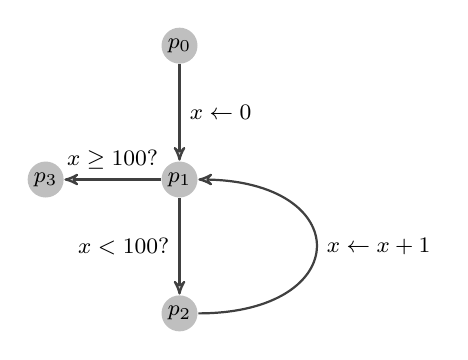
\begin{tikzpicture}[->,>=stealth',auto,node distance=1.7cm,
                    semithick,font=\footnotesize]

	\node[state] (n0) {$p_0$};
	\node[state] (n1) [below of=n0] {$p_1$};
	\node[state] (n2) [below of=n1] {$p_2$};
	\node[state] (n3) [left of=n1] {$p_3$};

  \path [transition] 
		(n0) edge              node {$x \gets 0$} (n1);
  \path [transition] 
        (n1) edge			   node [above] {$x \geq 100?$} (n3);
  \path [transition] 
        (n1) edge			   node [left] {$x < 100?$} (n2);
  \path [transition] 
        (n2) edge [out=0, in=0, distance=2cm] node [right] {$x \gets x+1$} (n1);

\end{tikzpicture}
   \end{column}
\end{columns}

\visible<2->{
\begin{eqnarray*}
X_1 =& \{x\ |\ x=0 \vee \exists x' \in X_2, x=x'+1 \} 
& \visible<3->{= \{ \only<1-2>{\}}\visible<3->{0} \only<3-4>{\}}\visible<5->{,1} \only<5-6>{\}} \visible<7->{,2,\dots}
 \only<7-8>{\}}\visible<9->{100} \only<9->{\}} }\\
X_2 =& \{x\ |\ x \in X_1 \wedge x < 100 \} 
& \visible<3->{= \only<3>{\emptyset} \only<4->{ \{0\only<6->{,1}
\only<8->{,2,\dots,99} \}}}
\end{eqnarray*}}
\end{frame}

\begin{frame}
\frametitle{Abstract Interpretation}

Cousot \& Cousot 1977

%\begin{tabular}{@{\textbullet~}p{0.8\textwidth}c@{}}
%Premier truc  & 2007-2010 \\
%Deuxième truc & 2000-2007 \\
%Troisième truc & 1997-2000 \\
%Quatrième truc & 1994-1997 \\
%Encore un truc bla bla & 1992-1994 \\
%\end{tabular}
\bigskip

Abstract domain to represent the set of possible states:
\begin{itemize}
\item Intervals \hfill
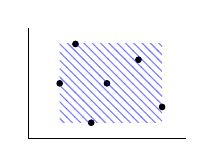
\begin{tikzpicture}[y=.1cm, x=.1cm,font=\footnotesize]

	%\draw[line] (0,0) -- (8,8) -- (16,0) -- cycle;

	\draw[fill=black] (4,7) circle (1pt);	
	\draw[fill=black] (6,12) circle (1pt);	
	\draw[fill=black] (8,2) circle (1pt);	
	\draw[fill=black] (10,7) circle (1pt);	
	\draw[fill=black] (14,10) circle (1pt);	
	\draw[fill=black] (17,4) circle (1pt);	

	\fill[polyhedra] (4,2) -- (4,12) -- (17,12) -- (17,2) -- cycle;
 	
	%axis
	\draw (0,0) -- coordinate (x axis mid) (20,0);
    \draw (0,0) -- coordinate (y axis mid) (0,14);
\end{tikzpicture} \hspace{3cm}~ 
\item Octagons
\hfill
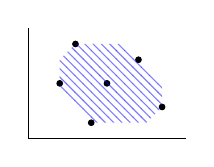
\begin{tikzpicture}[y=.1cm, x=.1cm,font=\footnotesize]

	%\draw[line] (0,0) -- (8,8) -- (16,0) -- cycle;

	\draw[fill=black] (4,7) circle (1pt);	
	\draw[fill=black] (6,12) circle (1pt);	
	\draw[fill=black] (8,2) circle (1pt);	
	\draw[fill=black] (10,7) circle (1pt);	
	\draw[fill=black] (14,10) circle (1pt);	
	\draw[fill=black] (17,4) circle (1pt);	

	\fill[polyhedra] (4,6) -- (4,10) -- (6,12) -- (12,12) 
	-- (17,7) -- (17,4) -- (15,2) -- (8,2) -- cycle;
 	
	%axis
	\draw (0,0) -- coordinate (x axis mid) (20,0);
    \draw (0,0) -- coordinate (y axis mid) (0,14);
\end{tikzpicture}   \hspace{3cm}~
\item Convex Polyhedra
\hfill
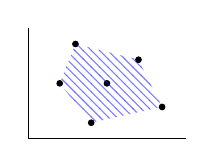
\begin{tikzpicture}[y=.1cm, x=.1cm,font=\footnotesize]

	%\draw[line] (0,0) -- (8,8) -- (16,0) -- cycle;

	\draw[fill=black] (4,7) circle (1pt);	
	\draw[fill=black] (6,12) circle (1pt);	
	\draw[fill=black] (8,2) circle (1pt);	
	\draw[fill=black] (10,7) circle (1pt);	
	\draw[fill=black] (14,10) circle (1pt);	
	\draw[fill=black] (17,4) circle (1pt);	

	\fill[polyhedra] (4,7) -- (6,12) -- (6,12) -- (14,10) 
	-- (17,4) -- (8,2) -- cycle;
 	
	%axis
	\draw (0,0) -- coordinate (x axis mid) (20,0);
    \draw (0,0) -- coordinate (y axis mid) (0,14);
\end{tikzpicture} \hspace{3cm}~

\end{itemize}

\bigskip

\visible<2->{$\Rightarrow$ Over-approximation of the set of states}
\end{frame}


\begin{frame}
\frametitle{Sources of Imprecision}
\begin{itemize}
\item<1-> Exact set that can't be expressed in the abstract domain
\item<2-> \alert<4>{Widening operator}
\begin{itemize}
\item Ensure termination
\item BUT: may induce huge imprecisions
\item Narrowing tends to recover some precision\ldots
\end{itemize}
\item<3-> \alert<4>{Consider paths that are unfeasible in reality}
\end{itemize}
\end{frame}

\begin{frame}
\frametitle{Summary}
\tableofcontents
\end{frame}


\section[Standard Approach]{Weakness of the Standard Approach}


\begin{frame}[containsverbatim]
  \frametitle{Example of Standard Abstract Interpretation}
\begin{columns}
\begin{column}{5cm}
\begin{lstlisting}
x = 0;
y = 0;
while (true) {
	if (x <= 50) 
		y++;
	else 
		y--;

	if (y < 0) break;
	x++;
}
\end{lstlisting}
\end{column}
\begin{column}{5cm}
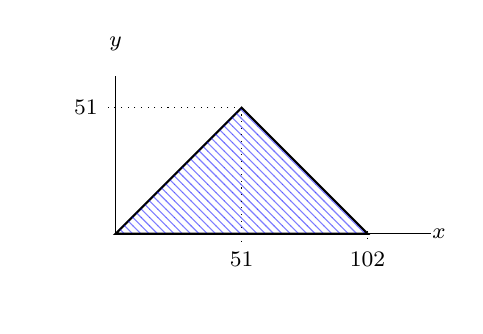
\begin{tikzpicture}[y=.2cm, x=.2cm,font=\footnotesize]

	\node (t1) at (-5,-4) {};
	\node (t2) at (13,11) {};
	\draw[line] (0,0) -- (8,8) -- (16,0) -- cycle;
	\fill[polyhedra] (0,0) -- (8,8) -- (16,0) -- cycle;
 	%axis
	\draw (0,0) -- coordinate (x axis mid) (20,0);
    \draw (0,0) -- coordinate (y axis mid) (0,10);

	%ticks and labels      
     		\draw [dotted](8,8) -- (-3pt,8) 
     			node[anchor=east] {$51$}; 
     		\draw [dotted] (8,8) -- (8,-3pt) 
     			node[anchor=north] {$51$}; 
     		\draw [dotted] (16,1pt) -- (16,-3pt) 
     			node[anchor=north] {$102$}; 

	\node[right=1.9cm] at (x axis mid) {$x$};
	\node[above=1.2cm] at (y axis mid) {$y$};
\end{tikzpicture} 
\end{column}
\end{columns}

\begin{itemize}
\item  $x$ and $y$ incremented during 51 iterations
\item  $x$ incremented and $y$ decremented during 51 iterations
\end{itemize}

\end{frame}

\begin{frame}
  \frametitle{Example of Standard Abstract Interpretation}

\begin{columns}
  \begin{column}{6cm}
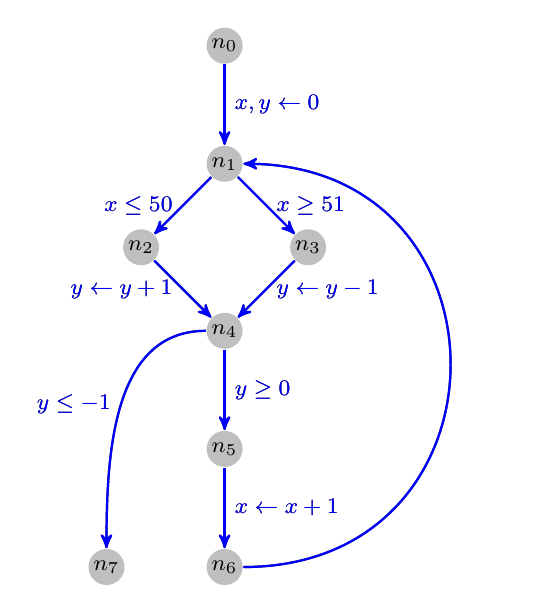
\begin{tikzpicture}[->,>=stealth',auto,node distance=1.5cm,
                    semithick,font=\footnotesize]

	\node[state] (n0) {$n_0$};
	\node[state] (n1) [below of=n0] {$n_1$};
	\node[state] (n2) [below left of=n1] {$n_2$};
	\node[state] (n3) [below right of=n1] {$n_3$};
	\node[state] (n4) [below left of=n3] {$n_4$};
	\node[state] (n5) [below of=n4] {$n_5$};
	\node[state] (n6) [below of=n5] {$n_6$};
	\node[state] (n7) [left of=n6] {$n_7$};

	\node (n8) [right of=n6] {};
	\node (n9) [right of=n1] {};

  \path<-1> [transition] 
		(n0) edge              node {$x,y \leftarrow 0$} (n1);
  \path<-2> [transition] 
        (n1) edge			   node [left] {$x \leq 50$} (n2);
  \path<-8> [transition] 
        (n1)  edge              node [right] {$x \geq 51$} (n3);
  \path<-3> [transition] 
        (n2) edge              node [left] {$y \leftarrow y+1$} (n4);
  \path<-9> [transition] 
        (n3) edge			   node [right] {$y \leftarrow y-1$} (n4);
  \path<-4> [transition] 
        (n4) edge			   node {$y \geq 0$} (n5);
  \path<-11> [transition] 
		(n4) edge  [out = 180, in=90] node [left] {$y \leq -1$} (n7);
  \path<-5> [transition] 
        (n5) edge              node {$x \leftarrow x+1$} (n6);
  \path<-6> [transition] 
        (n6) edge [out=0, in=0, distance=3.5cm] node {} (n1);

  \path<2-> [transition2] 
		(n0) edge              node {$x,y \leftarrow 0$} (n1);
  \path<3-> [transition2] 
        (n1) edge			   node [left] {$x \leq 50$} (n2);
  \path<9-> [transition2] 
        (n1)  edge              node [right] {$x \geq 51$} (n3);
  \path<4-> [transition2] 
        (n2) edge              node [left] {$y \leftarrow y+1$} (n4);
  \path<10-> [transition2] 
        (n3) edge			   node [right] {$y \leftarrow y-1$} (n4);
  \path<5-> [transition2] 
        (n4) edge			   node {$y \geq 0$} (n5);
  \path<12-> [transition2] 
		(n4) edge  [out = 180, in=90] node [left] {$y \leq -1$} (n7);
  \path<6-> [transition2] 
        (n5) edge              node {$x \leftarrow x+1$} (n6);
  \path<7-> [transition2] 
        (n6) edge [out=0, in=0, distance=3.5cm] node {} (n1);
\end{tikzpicture}
\end{column}
\begin{column}{5cm}
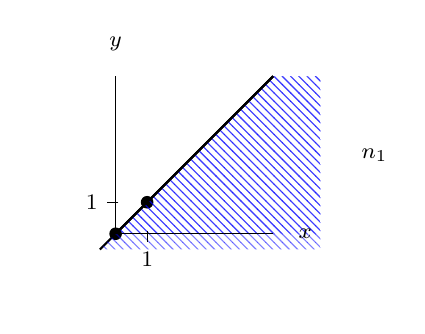
\begin{tikzpicture}[y=.2cm, x=.2cm,font=\footnotesize]

	\node (t1) at (-5,-4) {};
	\node (t2) at (13,11) {};
	\fill<2-7>[line] (0,0) circle (0.4);
	\fill<7>[line] (2,2) circle (0.4);
	\draw<8-10>[line] (0,0) -- (10,10) -- cycle;
	\draw<11-12>[line] (-1,-1) -- (10,10) -- cycle;
	\fill<11-12>[polyhedra] (-1,-1) -- (10,10) -- (13,10) -- (13,-1) -- (0,-1) -- cycle;
	\fill<13-14>[polyhedra] (0,0) -- (10,10) -- (13,10) -- (13,0) -- cycle;
	\draw<13-14>[line] (0,0) -- (10,10) -- cycle;

 	%axis
	\draw (0,0) -- coordinate (x axis mid) (10,0);
    \draw (0,0) -- coordinate (y axis mid) (0,10);

	%ticks and labels      
	\node[right=1.2cm] at (x axis mid) {$x$};
	\node[above=1.2cm] at (y axis mid) {$y$};

	\node[right=3cm] at (y axis mid) {$n_1$};

    \draw<7> (1pt,2) -- (-3pt,2) 
     	node[anchor=east] {1}; 
    \draw<7> (2,1pt) -- (2,-3pt) 
     	node[anchor=north] {1}; 

\end{tikzpicture} 
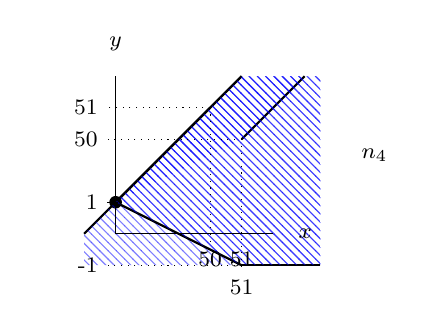
\begin{tikzpicture}[y=.2cm, x=.2cm,font=\footnotesize]

	\node (t1) at (-5,-4) {};
	\node (t2) at (13,11) {};
	\fill<4-9>[line] (0,2) circle (0.4);
	\fill<10-11>[polyhedra] (0,2) -- (8,10) -- (12,10) -- (8,6) --cycle;
	\draw<10-11>[line] (0,2) -- (6,8);
	\draw<10-11>[line] (8,6) -- (12,10);

	\draw<12-13>[line] (-2,0) -- (8,10);
	\fill<12-13>[polyhedra] (-2,-2) -- (-2,0) -- (8,10) -- (13,10) -- (13,-2) --
	 cycle;
	%\fill<12-13>[polyhedra] (-2,-2) -- (-2,0) -- (6,8) -- (6,-2) -- cycle;
	%\fill<12-14>[polyhedra] (8,6) -- (12,10) -- (13,10) -- (13,-2) -- (8,-2) -- cycle;

	\draw<14>[line] (0,2) -- (8,10);
	\draw<14>[line] (0,2) -- (8,-2);
	\draw<14>[line] (13,-2) -- (8,-2);
	\fill<14>[polyhedra] (0,2) -- (8,10) -- (13,10) -- (13,-2) -- (8,-2) -- cycle;
	%\fill<14>[polyhedra] (0,2) -- (6,8) -- (6,2) --  cycle;

 	%axis
	\draw (0,0) -- coordinate (x axis mid) (10,0);
    \draw (0,0) -- coordinate (y axis mid) (0,10);

	%labels      
	\node[right=1.2cm] at (x axis mid) {$x$};
	\node[above=1.2cm] at (y axis mid) {$y$};

	\node[right=3cm] at (y axis mid) {$n_4$};
	%ticks
     		\draw<4-> (1pt,2) -- (-3pt,2) 
     			node[anchor=east] {1}; 
     		\draw<14-> [dotted](8,-2) -- (-3pt,-2) 
     			node[anchor=east] {-1}; 
	
     		\draw<10-11> [dotted](6,8) -- (-3pt,8) 
     			node[anchor=east] {$51$}; 
     		\draw<10-11> [dotted] (8,6) -- (-3pt,6) 
     			node[anchor=east] {$50$}; 
     		\draw<10-11> [dotted](8,6) -- (8,-3pt) 
     			node[anchor=north] {$51$}; 
     		\draw<10-11> [dotted] (6,8) -- (6,-3pt) 
     			node[anchor=north] {$50$}; 
     		\draw<14-> [dotted](8,6) -- (8,-2.3) 
     			node[anchor=north] {$51$}; 
     		%\draw<14-> [dotted] (6,8) -- (6,-2.3) 
     		%	node[anchor=north] {$50$}; 
     		%\draw (2,1pt) -- (2,-3pt) 
     		%	node[anchor=north] {1}; 

\end{tikzpicture} 
\only<1-12>{Ascending iterations}
\only<13->{Descending iterations}
\end{column}
\end{columns}
\end{frame}


\section[Lookahead Widening]{Lookahead Widening Technique}

\begin{frame}
  \frametitle{Principle}

D. Gopan \& T. Reps, CAV 2006
\bigskip
\begin{itemize}
\item Separate loops into distinct phases.
\item Obtaining a solution for each loop phase before proceeding to the next.
\item Widening \& narrowing at each loop phase.
\begin{itemize}
\item Better precision
\end{itemize}
\end{itemize}
\end{frame}

\section[Path focusing]{Using SMT-Solving to Focus New Paths}

\begin{frame}
  \frametitle{Principle}

D. Monniaux \& L. Gonnord, SAS 2011
\bigskip
\begin{itemize}
\item Compute the fixpoint iterations on a multigraph
\item Take a set $P_R$ of nodes (in \alert{red}) cutting every loops
\item Distinguish all the paths between 2 nodes of $P_R$
\end{itemize}
\end{frame}


\begin{frame}
  \frametitle{Principle}
\begin{columns}
\begin{column}{5cm}
\centering
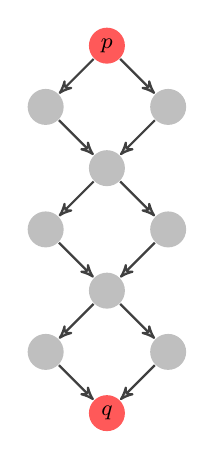
\begin{tikzpicture}[->,>=stealth',auto,node distance=1.1cm,
                    semithick,font=\footnotesize]

	\node[PRstate] (n0) {$p$};
	\node[state] (n1) [below left of=n0] {};
	\node[state] (n2) [below right of=n0] {};
	\node[state] (n3) [below right of=n1] {};
	\node[state] (n4) [below left of=n3] {};
	\node[state] (n5) [below right of=n3] {};
	\node[state] (n6) [below right of=n4] {};
	\node[state] (n7) [below left of=n6] {};
	\node[state] (n8) [below right of=n6] {};
	\node[PRstate] (n9) [below right of=n7] {$q$};

  \path [transition] 
		(n0) edge              node {} (n1);
  \path [transition] 
		(n0) edge              node {} (n2);
  \path [transition] 
		(n1) edge              node {} (n3);
  \path [transition] 
		(n2) edge              node {} (n3);
  \path [transition] 
		(n3) edge              node {} (n4);
  \path [transition] 
		(n3) edge              node {} (n5);
  \path [transition] 
		(n4) edge              node {} (n6);
  \path [transition] 
		(n5) edge              node {} (n6);
  \path [transition] 
		(n6) edge              node {} (n7);
  \path [transition] 
		(n6) edge              node {} (n8);
  \path [transition] 
		(n7) edge              node {} (n9);
  \path [transition] 
		(n8) edge              node {} (n9);
\end{tikzpicture}
\end{column} 
\begin{column}{5cm}
\visible<2->{
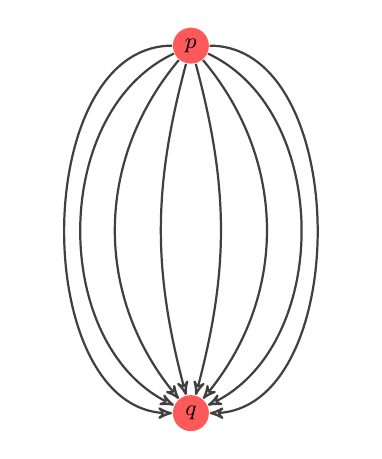
\begin{tikzpicture}[->,>=stealth',auto,node distance=1.1cm,
                    semithick,font=\footnotesize]

	\node[PRstate] (n0) {$p$};
	\node (n1) [below left of=n0] {};
	\node (n2) [below right of=n0] {};
	\node (n3) [below right of=n1] {};
	\node (n4) [below left of=n3] {};
	\node (n5) [below right of=n3] {};
	\node (n6) [below right of=n4] {};
	\node (n7) [below left of=n6] {};
	\node (n8) [below right of=n6] {};
	\node[PRstate] (n9) [below right of=n7] {$q$};

  \path [transition] 
		(n0) edge  [out=0, in=0]            node {} (n9);
  \path [transition] 
		(n0) edge  [out=180, in=180]        node {} (n9);
  \path [transition] 
		(n0) edge  [out=205, in=155]            node {} (n9);
  \path [transition] 
		(n0) edge  [out=230, in=130]            node {} (n9);
  \path [transition] 
		(n0) edge  [out=255, in=105]            node {} (n9);
  \path [transition] 
		(n0) edge  [out=-25, in=25]            node {} (n9);
  \path [transition] 
		(n0) edge  [out=-50, in=50]            node {} (n9);
  \path [transition] 
		(n0) edge  [out=-75, in=75]            node {} (n9);
\end{tikzpicture}
}
\end{column}
\end{columns}

\visible<3>{
	\centering
Exponential number of paths:
\begin{itemize}
\item We don't construct this graph explicitly
\item We use SMT-solving to find interesting paths
\end{itemize}
}

\end{frame}

\begin{frame}
  \frametitle{Reducing the Graph}

\begin{columns}
\begin{column}{5.5cm}
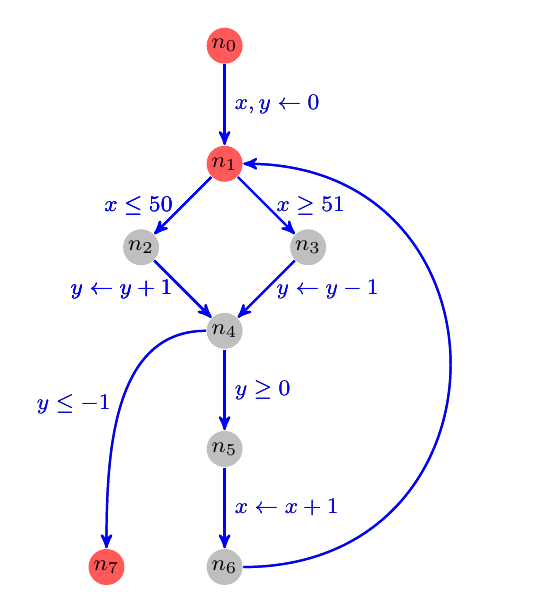
\begin{tikzpicture}[->,>=stealth',auto,node distance=1.5cm,
                    semithick,font=\footnotesize]

	\node[PRstate] (n0) {$n_0$};
	\node[PRstate] (n1) [below of=n0] {$n_1$};
	\node[state] (n2) [below left of=n1] {$n_2$};
	\node[state] (n3) [below right of=n1] {$n_3$};
	\node[state] (n4) [below left of=n3] {$n_4$};
	\node[state] (n5) [below of=n4] {$n_5$};
	\node[state] (n6) [below of=n5] {$n_6$};
	\node[PRstate] (n7) [left of=n6] {$n_7$};


  \path [transition] 
		(n0) edge              node {$x,y \leftarrow 0$} (n1);
  \path [transition] 
        (n1) edge			   node [left] {$x \leq 50$} (n2);
  \path [transition] 
        (n1)  edge              node [right] {$x \geq 51$} (n3);
  \path [transition] 
        (n2) edge              node [left] {$y \leftarrow y+1$} (n4);
  \path [transition] 
        (n3) edge			   node [right] {$y \leftarrow y-1$} (n4);
  \path [transition] 
        (n4) edge			   node {$y \geq 0$} (n5);
  \path [transition] 
		(n4) edge  [out = 180, in=90] node [left] {$y \leq -1$} (n7);
  \path [transition] 
        (n5) edge              node {$x \leftarrow x+1$} (n6);
  \path [transition] 
        (n6) edge [out=0, in=0, distance=3.5cm] node {} (n1);

  \path<3> [transition2] 
		(n0) edge              node {$x,y \leftarrow 0$} (n1);

  \path<4> [transition2] 
        (n1) edge			   node [left] {$x \leq 50$} (n2);
  \path<4> [transition2] 
        (n2) edge              node [left] {$y \leftarrow y+1$} (n4);
  \path<4-5> [transition2] 
        (n4) edge			   node {$y \geq 0$} (n5);
  \path<4-5> [transition2] 
        (n5) edge              node {$x \leftarrow x+1$} (n6);
  \path<4-5> [transition2] 
        (n6) edge [out=0, in=0, distance=3.5cm] node {} (n1);

  \path<5-6> [transition2] 
        (n1)  edge              node [right] {$x \geq 51$} (n3);
  \path<5-6> [transition2] 
        (n3) edge			   node [right] {$y \leftarrow y-1$} (n4);
  \path<6-> [transition2] 
		(n4) edge  [out = 180, in=90] node [left] {$y \leq -1$} (n7);

  \path<7> [transition2] 
        (n1) edge			   node [left] {$x \leq 50$} (n2);
  \path<7> [transition2] 
        (n2) edge              node [left] {$y \leftarrow y+1$} (n4);

\end{tikzpicture}
\end{column}
\begin{column}{5.5cm}
\visible<2->{
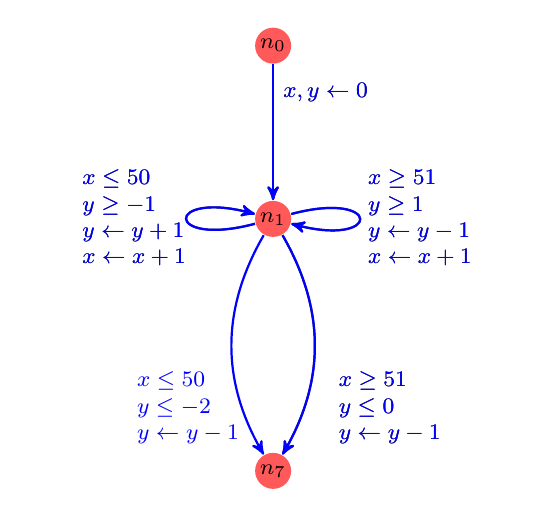
\begin{tikzpicture}[->,>=stealth',auto,node distance=3.2cm,
                    semithick,font=\footnotesize]

	\node[PRstate] (n0) {$n_0$};
	\node[PRstate] (n1) [below of=n0,yshift=1cm] {$n_1$};
	\node[PRstate] (n7) [below of=n1] {$n_7$};

	\node (n8) at (-3,0) {};
	\node (n8) at (3,0) {};

  \path<4-> [transition] 
		(n0) edge              node [yshift=5mm] {$x,y \leftarrow 0$} (n1);
  \path<7-> [transition] 
		(n1) edge    [bend left]  node [right,yshift=-0.8cm]  {$
		\begin{array}{l}
			x \geq 51 \\
			y \leq 0 \\
			y \leftarrow y-1
		\end{array}
		$} (n7);
%  \path<8-> [transition] 
%		(n1) edge    [bend right]  node [left,yshift=-0.8cm,xshift=4mm] {$
%		\begin{array}{l}
%			x \leq 50 \\
%			y \leq -2 \\
%			y \leftarrow y-1
%		\end{array}
%		$} (n7);
  \path<5-> [transition] 
		(n1) edge    [loop left,distance=1.2cm]  node [left,xshift=3mm] {$
		\begin{array}{l}
			x \leq 50 \\
			y \geq -1 \\
			y \leftarrow y+1 \\
			x \leftarrow x+1 
		\end{array}
		$} (n1);
  \path<6-> [transition] 
		(n1) edge    [loop right,distance=1.2cm]  node [right,xshift=-2mm] {$
		\begin{array}{l}
			x \geq 51 \\
			y \geq 1 \\
			y \leftarrow y-1 \\
			x \leftarrow x+1 
		\end{array}
		$} (n1);
  %\path [transition] 
  %      (n6) edge [out=0, in=0, distance=3.5cm] node {} (n1);
  \path<3> [transition2] 
		(n0) edge              node [yshift=5mm] {$x,y \leftarrow 0$} (n1);
  \path<6> [transition2] 
		(n1) edge    [bend left]  node [right,yshift=-0.8cm]  {$
		\begin{array}{l}
			x \geq 51 \\
			y \leq 0 \\
			y \leftarrow y-1
		\end{array}
		$} (n7);
  \path<7> [transition2] 
		(n1) edge    [bend right]  node [left,yshift=-0.8cm,xshift=4mm] {$
		\begin{array}{l}
			x \leq 50 \\
			y \leq -2 \\
			y \leftarrow y-1
		\end{array}
		$} (n7);
  \path<4> [transition2] 
		(n1) edge    [loop left,distance=1.2cm]  node [left,xshift=3mm] {$
		\begin{array}{l}
			x \leq 50 \\
			y \geq -1 \\
			y \leftarrow y+1 \\
			x \leftarrow x+1 
		\end{array}
		$} (n1);
  \path<5> [transition2] 
		(n1) edge    [loop right,distance=1.2cm]  node [right,xshift=-2mm] {$
		\begin{array}{l}
			x \geq 51 \\
			y \geq 1 \\
			y \leftarrow y-1 \\
			x \leftarrow x+1 
		\end{array}
		$} (n1);
\end{tikzpicture}
}
\end{column}
\end{columns}
\end{frame}

\begin{frame}
  \frametitle{Using SMT-Solving to Find New Paths}
\begin{itemize}
\item SMT formula $\rho$ expressing the semantics of the program
\begin{itemize}
\item Satisfiability Modulo Theory
\item Boolean + linear arithmetic
\end{itemize}
\item SMT-solver: decides the satisfiability and gives a model
\item $\rho$ contains reachability predicates
\end{itemize}
\bigskip
\begin{center}
Is there a path starting in the invariant candidate, that arrives in a
state outside the invariant?
\end{center}
\bigskip 
%To find a path from $p_1$ to $p_2$, ($p_1,p_2 \in P_R$) :
$$\rho  \wedge b_{p_1} \wedge x_1 \in X_{p_1} \wedge \bigvee_{p_2 \in succ(p_1)}
 (b_{p_2} \wedge x_2 \notin X_{p_2})$$

\footnotesize{
$b_{p_i}$: reachability predicate for $p_i$

$X_{p_i}$: abstract domain of node $p_i$
}
\end{frame}

\begin{frame}[containsverbatim]
	\frametitle{Example}
\begin{center}
\begin{lstlisting}
	int x = 0;
	int d = 1;
	
	while (true) {
		if (x == 0) d=1;
		if (x == 1000) d=-1;
		x +=d;
	}
\end{lstlisting}
\end{center}
\begin{itemize}
\item $x$ incremented until it is equal to $1000$,
\item $x$ decremented until it is equal to $0$,
\item restart\ldots
\end{itemize}

\end{frame}

\begin{frame}
  \frametitle{Example}
\begin{columns}
\begin{column}{7cm}
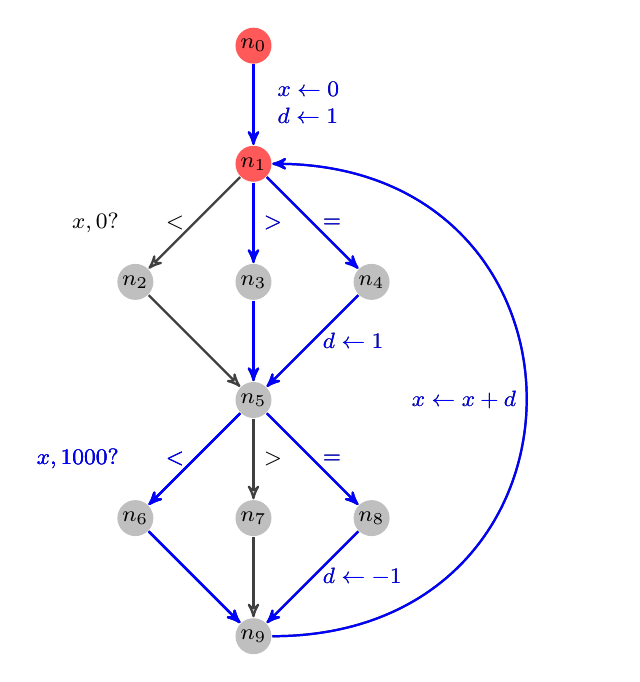
\begin{tikzpicture}[->,>=stealth',auto,node distance=1.5cm,
                    semithick,font=\footnotesize]
	\node[PRstate] (n0) {$n_0$};
	\node[PRstate] (n1) [below of=n0] {$n_1$};
	\node[state] (n3) [below of=n1] {$n_3$};
	\node[state] (n2) [left of=n3] {$n_2$};
	\node[state] (n4) [right of=n3] {$n_4$};
	\node[state] (n5) [below of=n3] {$n_5$};
	\node[state] (n7) [below of=n5] {$n_7$};
	\node[state] (n6) [left of=n7] {$n_6$};
	\node[state] (n8) [right of=n7] {$n_8$};
	\node[state] (n9) [below of=n7] {$n_9$};

  \path [transition] 
		(n0) edge              node  {$\begin{array}{l}
		x \leftarrow 0 \\
		d \leftarrow 1 
		\end{array}$} (n1);
  \path [transition] 
        (n1) edge			   node [left] {$x,0?$~ ~ ~ $<$} (n2);
  \path [transition] 
        (n1)  edge              node {$>$} (n3);
  \path [transition] 
        (n1)  edge              node [right] {$=$} (n4);
  \path [transition] 
        (n3) edge              node  {} (n5);
  \path [transition] 
        (n2) edge			   node {} (n5);
  \path [transition] 
        (n4) edge			   node [right] {$d \leftarrow 1$} (n5);
  \path [transition] 
        (n5) edge			   node [left] {$x,1000?$ ~ ~ ~$<$} (n6);
  \path [transition] 
        (n5) edge			   node {$>$} (n7);
  \path [transition] 
        (n5) edge			   node [right] {$=$} (n8);
  \path [transition] 
        (n6) edge              node {} (n9);
  \path [transition] 
        (n7) edge              node {} (n9);
  \path [transition] 
        (n8) edge              node [right] {$d \leftarrow -1$} (n9);
  \path [transition] 
        (n9) edge [out=0, in=0, distance=4.3cm] node [left] {$x \leftarrow x+d$} (n1);

  \path<1> [transition2] 
		(n0) edge              node  {$\begin{array}{l}
		x \leftarrow 0 \\
		d \leftarrow 1 
		\end{array}$} (n1);

  \path<2-3> [transition2] 
        (n1)  edge              node [right] {$=$} (n4);
  \path<2-3> [transition2] 
        (n4) edge			   node [right] {$d \leftarrow 1$} (n5);
  \path<2-5> [transition2] 
        (n5) edge			   node [left] {$x,1000?$ ~ ~ ~$<$} (n6);
  \path<2-5> [transition2] 
        (n6) edge              node {} (n9);
  \path<2-> [transition2] 
        (n9) edge [out=0, in=0, distance=4.3cm] node [left] {$x \leftarrow x+d$} (n1);
  \path<4-> [transition2] 
        (n1) edge			   node {$>$} (n3);
  \path<4-> [transition2] 
        (n3) edge			   node {} (n5);
	
  \path<6-7> [transition2] 
        (n5) edge			   node [right] {$=$} (n8);
  \path<6-7> [transition2] 
        (n8) edge              node [right] {$d \leftarrow -1$} (n9);
  \path<8-> [transition2] 
        (n5) edge			   node [left] {$x,1000?$ ~ ~ ~$<$} (n6);
  \path<8-> [transition2] 
        (n6) edge              node {} (n9);
\end{tikzpicture}
\end{column}
\begin{column}{5cm}
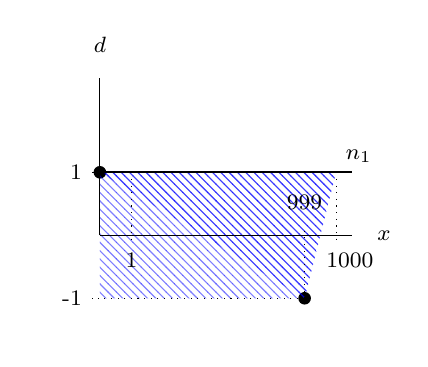
\begin{tikzpicture}[y=.2cm, x=.2cm,font=\footnotesize]

	\fill<-1>[line] (0,4) circle (0.4);
	\fill<6->[line] (13,-4) circle (0.4);
	\fill<7>[polyhedra] (13,-4) -- (0,4) -- (15,4) -- cycle;
	\fill<8->[polyhedra] (13,-4) -- (0,-4) -- (0,4) -- (15,4) -- cycle;
	\draw<3>[line] (0,4) -- (2,4) -- cycle;
	\draw<2>[line] (0,4) -- (16,4) -- cycle;
	\draw<4>[line] (0,4) -- (16,4) -- cycle;
	\draw<5->[line] (0,4) -- (15,4) -- cycle;

 	%axis
	\draw (0,0) -- coordinate (x axis mid) (16,0);
    \draw (0,0) -- coordinate (y axis mid) (0,10);

	%ticks and labels      
	\node[right=1.8cm] at (x axis mid) {$x$};
	\node[above=1.2cm] at (y axis mid) {$d$};
	
	\node at (-4,-6) {};

     		\draw<1-> (1pt,4) -- (-3pt,4) 
     			node[anchor=east] {1}; 
     		\draw<6-> [dotted] (13,-4) -- (-3pt,-4) 
     			node[anchor=east] {-1}; 
     		\draw<3-3> [dotted] (2,4) -- (2,-3pt) 
     			node[anchor=north] {1}; 
     		\draw<5-> [dotted] (15,4) -- (15,-3pt) 
     			node[anchor=north,xshift=5pt] {1000}; 
     		\draw<6-> [dotted] (13,-4) -- (13,3pt) 
     			node[anchor=north,yshift=15pt] {999}; 

	\node[right=3cm] at (y axis mid) {$n_1$};
\end{tikzpicture} 

\visible<9>{
\begin{itemize}
\item 9 paths from $n_1$ to $n_1$
\item Only 3 are computed
\end{itemize}
}
\end{column}
\end{columns}
\end{frame}


\section[Results]{Results}

\begin{frame}
  \frametitle{What is Done (1)}

Implementation of an analyzer
\begin{itemize}
\item 
Using:
\begin{itemize}
\item LLVM compiler infrastructure
\item Apron numerical abstract domain library
\item SMT-solvers Yices and Microsoft Z3
\end{itemize}

\item  Both techniques implemented
\begin{itemize}
\item Lookahead widening
\item Path Focusing
\end{itemize}

\item Evaluation and comparison
\end{itemize}
\end{frame}



\begin{frame}
\frametitle{Benchmark Results}

\begin{itemize}
\item $\approx$ 50 test-cases
\item $\approx$ 30 benchmarks (cbench)
\item $\approx$ 10 GNU projects:
\end{itemize}

\begin{table}
\centering \small
\begin{tabular}{|c||r|r|r|} \hline 
Benchmark  & Lookahead Widening & Path Focusing & None better \\
\hline \hline
Gawk		& 3		& 4		& 284  \\ \hline
Gnuchess	& 33	& 22	& 1506  \\ \hline
Gnugo		& 35	& 105	& 1303  \\ \hline
Grep		& 3		& 4		& 323  \\ \hline
Gzip		& 3		& 9		& 189  \\ \hline
Make		& 11	&  7	& 457  \\ \hline
Tar			& 5		& 16	& 555  \\ \hline
Wget		& 12	& 8		& 715  \\ \hline \hline
TOTAL		& 105	& 175	& 5332	\\ \hline
\end{tabular}
\caption{Result of the analysis of various open-source projects.}
\label{opensource}
\end{table}
\end{frame}

\begin{frame}
\frametitle{What is Done (2)}

\begin{itemize}
\item Correction of some oversights in Path Focusing technique
\item Ideas to refine the algorithm
\begin{itemize}
\item Combine both techniques
\item Compute disjunctive invariants (Gulwani \& Zuleger, PLDI 2010)
\end{itemize}
\end{itemize}
\end{frame}

\begin{frame}
  \frametitle{Future Work}
\begin{itemize}
\item Choice of $P_R$ (red points)
\item Programs with non-linear arithmetic
\item Analysis with pointers
\item Overflows analysis
\end{itemize}
\end{frame}



\begin{frame}
\begin{center}
Thank you!

\begin{columns}
\begin{column}{5cm}
\includegraphics[width=4cm]{ariane}
\end{column}
\begin{column}{4cm}
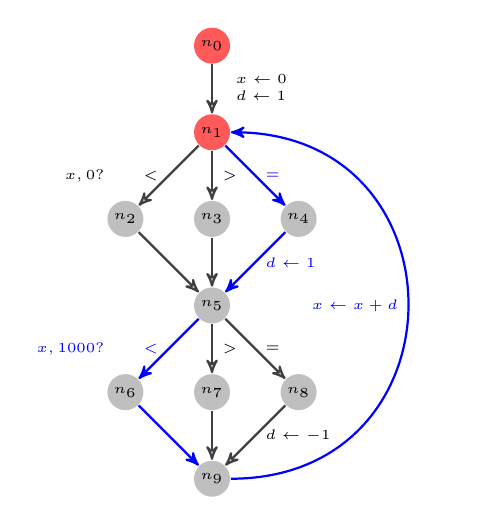
\begin{tikzpicture}[->,>=stealth',auto,node distance=1.1cm,
                    semithick,font=\tiny]
	\node[PRstate] (n0) {$n_0$};
	\node[PRstate] (n1) [below of=n0] {$n_1$};
	\node[state] (n3) [below of=n1] {$n_3$};
	\node[state] (n2) [left of=n3] {$n_2$};
	\node[state] (n4) [right of=n3] {$n_4$};
	\node[state] (n5) [below of=n3] {$n_5$};
	\node[state] (n7) [below of=n5] {$n_7$};
	\node[state] (n6) [left of=n7] {$n_6$};
	\node[state] (n8) [right of=n7] {$n_8$};
	\node[state] (n9) [below of=n7] {$n_9$};

  \path [transition] 
		(n0) edge              node  {$\begin{array}{l}
		x \leftarrow 0 \\
		d \leftarrow 1 
		\end{array}$} (n1);
  \path [transition] 
        (n1) edge			   node [left] {$x,0?$~ ~ ~ $<$} (n2);
  \path [transition] 
        (n1)  edge              node {$>$} (n3);
  \path [transition2] 
        (n1)  edge              node [right] {$=$} (n4);
  \path [transition] 
        (n3) edge              node  {} (n5);
  \path [transition] 
        (n2) edge			   node {} (n5);
  \path [transition2] 
        (n4) edge			   node [right] {$d \leftarrow 1$} (n5);
  \path [transition2] 
        (n5) edge			   node [left] {$x,1000?$ ~ ~ ~$<$} (n6);
  \path [transition] 
        (n5) edge			   node {$>$} (n7);
  \path [transition] 
        (n5) edge			   node [right] {$=$} (n8);
  \path [transition2] 
        (n6) edge              node {} (n9);
  \path [transition] 
        (n7) edge              node {} (n9);
  \path [transition] 
        (n8) edge              node [right] {$d \leftarrow -1$} (n9);
  \path [transition2] 
        (n9) edge [out=0, in=0, distance=3cm] node [left] {$x \leftarrow x+d$} (n1);
\end{tikzpicture}
\end{column}
\end{columns}

\end{center}
\end{frame}


\backupbegin

\begin{frame}
\frametitle{Overflows Analysis}
Semantics of the addition $x+y$:
\begin{center}
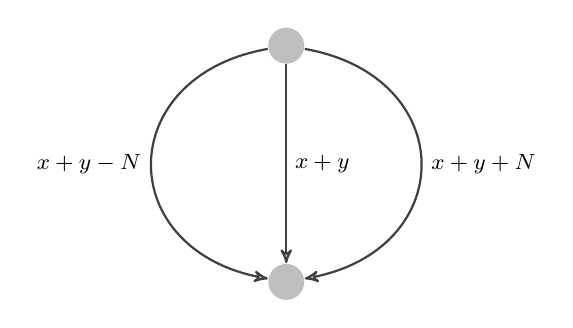
\begin{tikzpicture}[->,>=stealth',auto,node distance=3cm,
                    semithick,font=\footnotesize]
	\node[state] (n0) {};
	\node[state] (n1) [below of=n0] {};

	\path [transition] 
		(n0) edge   node [xshift=-0.2mm] {$x+y$} (n1)
		(n0) edge [in=170,out=190,distance=2cm]  node [left] {$x+y-N$} (n1)
		(n0) edge [in=10,out=-10,distance=2cm]  node [right] {$x+y+N$} (n1);
\end{tikzpicture}
\end{center}
\end{frame}
\begin{frame}

\frametitle{Pointer Analysis}
Pointer $p$ can point to $x$, $y$, or $z$: 
\begin{center}
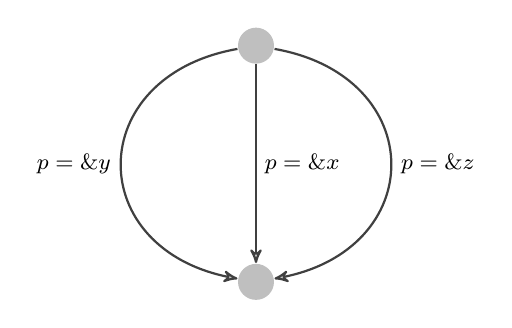
\begin{tikzpicture}[->,>=stealth',auto,node distance=3cm,
                    semithick,font=\footnotesize]
	\node[state] (n0) {};
	\node[state] (n1) [below of=n0] {};

	\path [transition] 
		(n0) edge   node [xshift=-0.2mm] {$p=\&x$} (n1)
		(n0) edge [in=170,out=190,distance=2cm]  node [left] {$p=\&y$} (n1)
		(n0) edge [in=10,out=-10,distance=2cm]  node [right] {$p=\&z$} (n1);
\end{tikzpicture}
\end{center}
\end{frame}

\begin{frame}[containsverbatim]
\frametitle{Example of $\rho$ Formula}
{\footnotesize
\begin{columns}
\begin{column}{6.2cm}
\begin{C}
(and 
 (= bd_0 false)
 (= t_0_1 bs_0)
 (or (not bd_0) true)
 (= b_5 t_1_5)
 (= x_%6 (+ x_y.0 -1))
 (= t_5_7 b_5)
 (or (not b_5) true)
 (= b_3 t_1_3)
 (= x_%4 (+ x_y.0 1))
 (= t_3_7 b_3)
 (or (not b_3) true)
 (= b_7
   (or t_5_7 t_3_7))
 (= t_7_9 (and b_7 (< x_y.1 0)))
 (= t_7_10
   (and b_7 (not (< x_y.1 0))))
 (or (not b_7)
   (= x_y.1 (ite t_3_7 x_%4 
                        x_%6)))
\end{C}
\end{column}
\begin{column}{9cm}
\begin{C}
 (= b_10 t_7_10)
 (= x_%11 (+ x_x.0 1))
 (= t_10_1 b_10)
 (or (not b_10) true)
 (= bd_1
   (or t_10_1 t_0_1))
 (= t_1_3 
   (and bs_1 (<= x_x.0 50)))
 (= t_1_5
   (and bs_1 (not (<= x_x.0 50))))
 (or (not bd_1)
   (and (= x'_x.0 
         (ite t_0_1 0 x_%11))
        (= x'_y.0 
         (ite t_0_1 0 x_y.1))))
 (= b_9 t_7_9)
 (= t_9_12 b_9)
 (or (not b_9) true)
 (= bd_12 t_9_12)
 (or (not bd_12) true))
\end{C}
\end{column}
\end{columns}
}
\end{frame}

\begin{frame}
\frametitle{Example of bad Results With Path Focusing}
\begin{figure}[!h]
\centering
\tikzstyle{rstate}=[rectangle,fill=black!25,minimum size=13pt,inner sep=0pt]
\tikzstyle{rprstate}=[rectangle,fill=red!65,minimum size=13pt,inner sep=0pt]
\begin{tikzpicture}[->,>=stealth',auto,node distance=1.8cm,
                    semithick,font=\footnotesize]

	\node[rstate] (n0) {$p_0$};
	\node[rprstate] (n1) [below of=n0] {\begin{tabular}{l}
	$p_1$: \\
	$i \gets \Phi(0,i')$
	\end{tabular}};
	\node[rprstate] (n2) [below left of=n1] {$p_2$};
	\node[rstate] (n3) [below right of=n2] {$p_3$};

  \path [transition] 
		(n0) edge              node {} (n1);
  \path [transition] 
        (n1) edge			   node [left] {$i \leq 50$} (n2);
  \path [transition] 
        (n2) edge	[loop left, distance=2cm]	   node  {} (n2);
  \path [transition] 
        (n2) edge			   node  {} (n3);
  \path [transition] 
        (n3) edge			   node [right] {$i' \gets i+1$} (n1);
\end{tikzpicture}
\end{figure}
\end{frame}

\backupend

\end{document}

%%% Local Variables:
%%% mode: latex
%%% TeX-master: t
%%% ispell-local-dictionary: "american"
%%% End:
